\documentclass{beamer}
\beamertemplatenavigationsymbolsempty
\usepackage{tikz}
\begin{document}

\begin{frame}{More techniques for computing chromatic polynomials}
  \begin{block}{Main goal: two new bits}
    \begin{itemize}
    \item Use induction to calculate $P_G(k)$ for a family of graphs.
      We'll do $C_n$
    \item Gluing formulas for graphs that are nearly disconnected
 \end{itemize}
    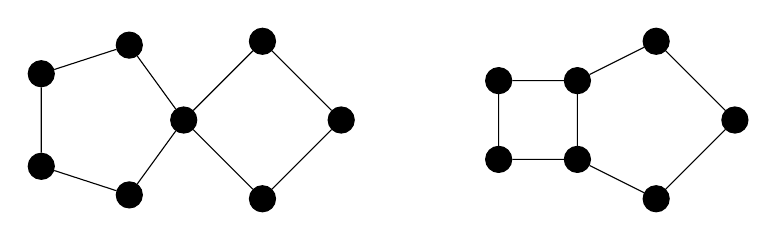
\begin{tikzpicture}[every node/.style={circle, fill, draw}]
      \begin{scope}[yshift=.5cm]
      \node (1) at (0:1) {};
      \node (2) at (72:1) {};
      \node (3) at (144:1) {};
      \node (4) at (216:1) {};
      \node (5) at (288:1) {};
      \node (6) at (2,1) {};
      \node (7) at (3, 0) {};
      \node (8) at (2,-1) {};
      \draw (1)--(2)--(3)--(4)--(5)--(1)--(6)--(7)--(8)--(1);
       
        \end{scope}

      
      \begin{scope}[xshift=5cm]
      \node (1) at (0,0) {};
      \node (2) at (0,1) {};
      \node (3) at (1,1) {};
      \node (4) at (1,0) {};
      \node (5) at (2,1.5) {};
      \node (6) at (3,.5) {};
      \node (7) at (2, -.5) {};
      \draw (3)--(2)--(1)--(4)--(3)--(5)--(6)--(7)--(4);
\end{scope}
      \end{tikzpicture}

    The graphs above glued from $C_4$ and $C_5$.
\end{block}
\begin{block}{If we have time:}
  Compute $P_G(k)$ for a relatively complicated graph $G$.
\end{block}
\end{frame}    



\begin{frame}{Calculating the chromatic polynomial of $C_n$}
  Let $e$ be any edge of $C_n$.  Then:
  \begin{itemize}
  \item $C_n/e \cong C_{n-1}$
  \item $C_n\setminus e=P_n$, a tree, so $P_{P_n}(k)=k(k-1)^{n-1}$
  \end{itemize}

  So we should be able to find $P_{C_n}(k)$ using induction, but need to ``guess'' the formula first.
 \begin{align*}
    P_4(k)= & k^4-4k^3+6k^2-3k \\
P_5(k)= & k^5-5k^4+10k^3-10k^2+4k \\
P_6(k)= & k^6-6k^5+15k^4-20k^3+15k^3-5k \\
P_7(k)= & k^7-7k^6+21k^5-35k^4+35k^3-21k^2+6k
    \end{align*}
\begin{block}{Looks like:}
$$P_n(k)=(k-1)^n+(-1)^n(k-1)$$
  \end{block}
\end{frame}

\begin{frame}{Inductive proof that $P_{C_n}(k)=(k-1)^n+(-1)^n(k-1)$}
  \begin{block}{Base case: $n=3$}
Plug in $n=3$, get $k(k-1)(k-2)=P_{C_3}(k)$.
  \end{block}

  \begin{block}{Inductive step:}
   Get to assume: $P_{C_{n-1}}(k)=(k-1)^{n-1}+(-1)^{n-1}(k-1)$

    \begin{itemize}
      \item $C_n\setminus e=P_n$, a tree, so $P_{C_{n-1}\setminus e}=k(k-1)^{n-1}$
      \item $C_n/e=C_{n-1}$, so $P_{C_n/e}(k)=(k-1)^{n-1}+(-1)^n(k-1)$.
        \end{itemize}
\end{block}
    \begin{block}{Plugging into deletion-contraction:}   \begin{align*}
      P_{C_n}(k)&=P_{C_n\setminus e}(k)-P_{C_n/e}(k) \\
      &=k(k-1)^{n-1}-\left[(k-1)^{n-1}+(-1)^{n-1}(k-1)\right] \\
      &=k(k-1)^{n-1}-(k-1)^{n-1}-(-1)^{n-1}(k-1) \\
      &=(k-1)^{n-1}\left[k-1\right] +(-1)^n(k-1) \\
      &=(k-1)^n+(-1)^n(k-1)
    \end{align*}
    \end{block}

\end{frame}

\begin{frame}{Gluing formulas: intro}
  \begin{lemma} If $G$ is the disjoint union of $G_1$ and $G_2$, then
    $$P_G(k)=P_{G_1}(k)P_{G_2}(k)$$
    \end{lemma}
\begin{proof} Colouring $G$ is exactly the same as colouring $G_1$ and $G_2$ independently.
\end{proof}


\begin{block}{Gluing formulas: when $G$ isn't \emph{quite} a disjoint union}
  Idea: Colour $G_1$, then extend to a colouring of $G_2$.
\end{block}
\end{frame}
\begin{frame}{Gluing formulas: statements}
    \begin{lemma}If $G$ is made by gluing $G_1$ and $G_2$ along a vertex $v$, then:

      $$P_G(k)=\frac{1}{k}P_{G_1}(k)P_{G_2}(k)$$
      \end{lemma}



    
    \begin{proof}First colour $G_1$ in any of the $P_{G_1}(k)$ ways.  Now, vertex $v$ of $G_2$ is already coloured, but none of the rest.  Since the colours are interchangable, exactly $1/k$ of the ways of colouring $G_2$ will have the right colour at $v$.
\end{proof}
    \begin{lemma}
      If $G$ is made by gluing $G_1$ and $G_2$ along an edge $e$, then $$P_G(k)=\frac{1}{k(k-1)} P_{G_1}(k)P_{G_2}(k)$$
\end{lemma}


  
\end{frame}


\begin{frame}{Find $P_G(k)$ for the following graphs}
  \centering
  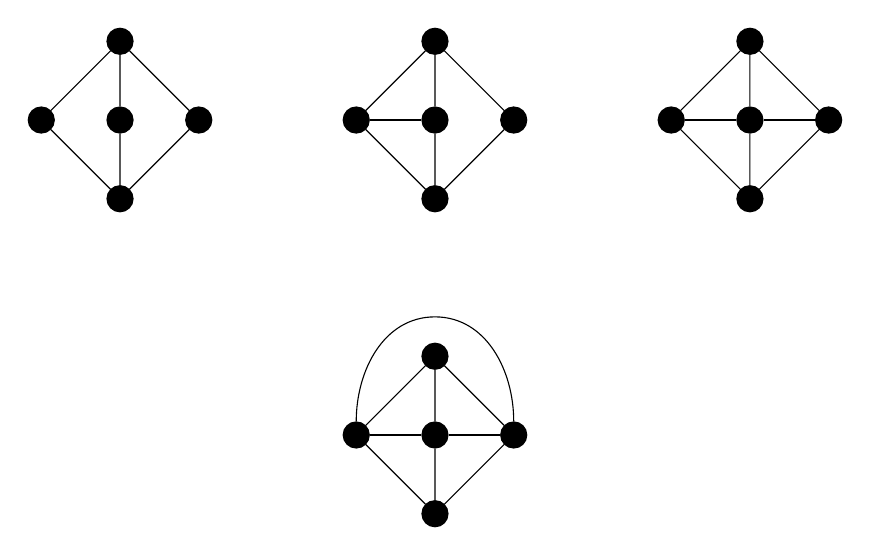
\begin{tikzpicture}[every node/.style={circle, fill, draw}]
    \begin{scope}
      \node (1) at (1,1) {};
      \node (2) at (0,0) {};
      \node (3) at (1,0) {};
      \node (4) at (2,0) {};
      \node (5) at (1,-1) {};
      \draw (1)--(2)--(5)--(3)--(1)--(4)--(5);
    \end{scope}

      \begin{scope}[xshift=4cm]
      \node (1) at (1,1) {};
      \node (2) at (0,0) {};
      \node (3) at (1,0) {};
      \node (4) at (2,0) {};
      \node (5) at (1,-1) {};
      \draw (1)--(2)--(5)--(3)--(1)--(4)--(5);
\draw (2)--(3);
      \end{scope}

        \begin{scope}[xshift=8cm]
      \node (1) at (1,1) {};
      \node (2) at (0,0) {};
      \node (3) at (1,0) {};
      \node (4) at (2,0) {};
      \node (5) at (1,-1) {};
      \draw (1)--(2)--(5)--(3)--(1)--(4)--(5);
      \draw (2)--(3)--(4);
        \end{scope}
    
  \begin{scope}[xshift=4cm, yshift=-4cm]
      \node (1) at (1,1) {};
      \node (2) at (0,0) {};
      \node (3) at (1,0) {};
      \node (4) at (2,0) {};
      \node (5) at (1,-1) {};
      \draw (1)--(2)--(5)--(3)--(1)--(4)--(5);
      \draw (2)--(3)--(4);
      \draw (2) to[out=90, in=180] (1,1.5) to[out=0,in=90] (4);

  \end{scope}

    \end{tikzpicture}


  \end{frame}

\end{document}
